\documentclass[tikz,border=5mm]{standalone}
\begin{document}
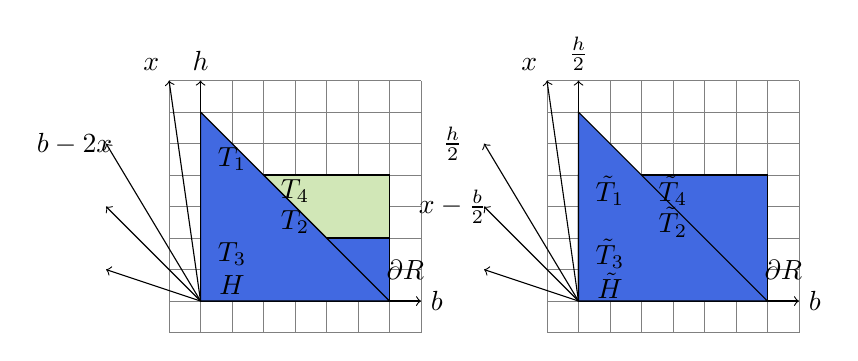
\begin{tikzpicture}[scale=0.8]
% Set colors
\definecolor{myred}{RGB}{255, 174, 96}
\definecolor{mygreen}{RGB}{139, 195, 74}
\definecolor{myblue}{RGB}{65, 105, 225}
\definecolor{mypurple}{RGB}{149, 109, 162}
% Draw grid and axis
\draw[help lines,xstep=0.5,ystep=0.5] (-0.5,-0.5) grid (3.5,3.5);
\draw[->] (0,0)--(3.5,0) node[right]{$b$};
\draw[->] (0,0)--(0,3.5) node[above]{$h$};
\draw[->] (0,0)--(-0.5,3.5) node[above left]{$x$};
\draw[->] (0,0)--(-1.5,1.5);
\draw[->] (0,0)--(-1.5,0.5);
\draw[->] (0,0)--(-1.5,2.5);
\node at (-2,2.5){$b-2x$};
% Draw the boxes
\draw[fill=mygreen!40] (0,0)--(3,0)--(3,2)--(0,2)--cycle;
\draw[fill=mygreen!20] (0,0)--(3,0)--(1,2)--(0,2)--cycle;
\draw[fill=myblue] (0,0)--(3,0)--(3,1)--(0,1)--cycle;
\draw[fill=myblue] (0,0)--(3,0)--(0,3)--(0,2)--cycle;
\node at (0.5,0.25){$H$};
\node at (1.5,1.25){$T_{2}$};
\node at (0.5,2.25){$T_{1}$};
\node at (0.5,0.75){$T_{3}$};
\node at (1.5,1.75){$T_{4}$};
\node at (3.25,0.5){$\partial R$};
% Draw the grid and axis for the other case
\begin{scope}[shift={(6,0)}]
\draw[help lines,xstep=0.5,ystep=0.5] (-0.5,-0.5) grid (3.5,3.5);
\draw[->] (0,0)--(3.5,0) node[right]{$b$};
\draw[->] (0,0)--(0,3.5) node[above]{$\frac{h}{2}$};
\draw[->] (0,0)--(-0.5,3.5) node[above left]{$x$};
\draw[->] (0,0)--(-1.5,2.5);
\draw[->] (0,0)--(-1.5,1.5);
\draw[->] (0,0)--(-1.5,0.5);
\node at (-2,2.5){$\frac{h}{2}$};
\node at (-2,1.5){$x-\frac{b}{2}$};
% Draw the boxes
\draw[fill=mygreen!20] (0,0)--(3,0)--(1,2)--(0,2)--cycle;
\draw[fill=mygreen!40] (0,0)--(3,0)--(3,1)--(0,1)--cycle;
\draw[fill=myblue] (0,0)--(3,0)--(3,2)--(0,2)--cycle;
\draw[fill=myblue] (0,0)--(3,0)--(0,3)--(0,2)--cycle;
\node at (0.5,0.25){$\tilde{H}$};
\node at (1.5,1.25){$\tilde{T}_{2}$};
\node at (0.5,1.75){$\tilde{T}_{1}$};
\node at (0.5,0.75){$\tilde{T}_{3}$};
\node at (1.5,1.75){$\tilde{T}_{4}$};
\node at (3.25,0.5){$\partial R$};
\end{scope}
\end{tikzpicture}
\end{document}